\documentclass[12pt,a4paper]{article}

% ─── Page Layout ───────────────────────────────────────────────────────────────
\usepackage[a4paper, margin=0.8in, headheight=14pt]{geometry}

% ─── Fonts (XeLaTeX) ───────────────────────────────────────────────────────────
\usepackage{fontspec}
\usepackage{unicode-math}
\setmainfont{TeX Gyre Pagella}
\setmonofont[Scale=0.88]{TeX Gyre Cursor}
\setmathfont{Latin Modern Math}

% ─── Packages ──────────────────────────────────────────────────────────────────
\usepackage{xcolor}
\usepackage{colortbl}
\usepackage{titlesec}
\usepackage{enumitem}
\usepackage{tabularx}
\usepackage{booktabs}
\usepackage{array}
\usepackage{amsmath}
\usepackage{tikz}
\usetikzlibrary{shapes.geometric, arrows.meta, positioning, calc, fit, decorations.pathreplacing, patterns}
\usepackage{tcolorbox}
\tcbuselibrary{skins, breakable}
\usepackage{hyperref}
\usepackage{fancyhdr}
\usepackage{graphicx}
\usepackage{microtype}
\hyphenpenalty=10000
\exhyphenpenalty=10000
\sloppy
\usepackage{caption}
\usepackage{setspace}
\usepackage{multirow}
\usepackage{tocloft}

% ─── Q&A helper ────────────────────────────────────────────────────────────────
\newcommand{\Q}[1]{\textbf{#1}\par\noindent\ignorespaces}

% ─── Colour Palette ────────────────────────────────────────────────────────────
\definecolor{myred}{RGB}{196,30,58}
\definecolor{mydark}{RGB}{30,30,50}
\definecolor{mygreen}{RGB}{14,120,80}
\definecolor{myteal}{RGB}{0,130,140}
\definecolor{myamber}{RGB}{180,100,0}
\definecolor{mypurple}{RGB}{100,30,160}
\definecolor{mygray}{RGB}{246,247,249}
\definecolor{mgframe}{RGB}{180,185,200}
\definecolor{watermark}{RGB}{145,150,170}
\definecolor{hdrred}{RGB}{250,232,235}
\definecolor{hdrgreen}{RGB}{220,244,233}
\definecolor{hdrteal}{RGB}{220,242,244}
\definecolor{hdramber}{RGB}{253,242,215}
\definecolor{hdrpurple}{RGB}{238,228,255}
\definecolor{hdrgray}{RGB}{238,240,245}
\definecolor{rowalt}{RGB}{250,251,253}

% ─── Section Formatting ────────────────────────────────────────────────────────
\titleformat{\section}{\large\bfseries\color{myred}}{\thesection.}{0.5em}{}[\vspace{1pt}{\color{myred}\rule{\linewidth}{0.8pt}}]
\titleformat{\subsection}{\normalsize\bfseries\color{myteal}}{\thesubsection}{0.5em}{}
\titlespacing*{\section}{0pt}{18pt}{7pt}
\titlespacing*{\subsection}{0pt}{11pt}{4pt}

% ─── Paragraph ─────────────────────────────────────────────────────────────────
\setlength{\parindent}{0pt}
\setlength{\parskip}{4pt}

% ─── TOC Styling ───────────────────────────────────────────────────────────────
\renewcommand{\cfttoctitlefont}{\large\bfseries\color{myred}}
\renewcommand{\cftaftertoctitle}{\par\noindent{\color{myred}\rule{\linewidth}{0.8pt}}}
\setlength{\cftbeforetoctitleskip}{0pt}
\setlength{\cftaftertoctitleskip}{6pt}
\renewcommand{\cftsecfont}{\normalsize\bfseries\color{mydark}}
\renewcommand{\cftsecpagefont}{\normalsize\bfseries\color{mydark}}
\renewcommand{\cftsecleader}{\cftdotfill{\cftdotsep}}
\setlength{\cftbeforesecskip}{7pt}
\renewcommand{\cftsubsecfont}{\small\color{mydark}}
\renewcommand{\cftsubsecpagefont}{\small\color{mydark}}
\setlength{\cftbeforesubsecskip}{3pt}
\setlength{\cftsubsecindent}{1.4em}

% ─── Table helpers ─────────────────────────────────────────────────────────────
\renewcommand{\arraystretch}{1.45}
\setlength{\tabcolsep}{6pt}
\arrayrulecolor{mydark}
\newcolumntype{B}[1]{>{\small\bfseries\raggedright\arraybackslash}m{#1}}
\newcolumntype{Y}{>{\small\raggedright\arraybackslash}X}
\renewcommand{\tabularxcolumn}[1]{m{#1}}

% ─── Header / Footer ───────────────────────────────────────────────────────────
\pagestyle{fancy}
\fancyhf{}
\fancyhead[L]{\small\color{myred}\textbf{OE-EC803A}\;\color{mydark}--- Internet of Things}
\fancyhead[R]{\small\color{myteal}\textbf{Module 2 Notes}}
\fancyfoot[C]{\small\color{mydark}\thepage}
\fancyfoot[R]{\small\color{watermark}\textit{\copyright\ Biraj Sarkar}}
\renewcommand{\headrulewidth}{0.5pt}
\renewcommand{\footrulewidth}{0.3pt}

% ─── Hyperref ──────────────────────────────────────────────────────────────────
\hypersetup{colorlinks=true, linkcolor=myteal, urlcolor=myteal,
  pdfauthor={Biraj Sarkar}, pdftitle={OE-EC803A --- Module 2 Notes}}

% ─── tcolorbox styles ──────────────────────────────────────────────────────────
\tcbset{
  tikzbox/.style={colback=mygray, colframe=mgframe, boxrule=0.6pt, arc=4pt,
    left=8pt, right=8pt, top=6pt, bottom=6pt,
    colbacktitle=mgframe, coltitle=mydark, fonttitle=\small\bfseries},
  defbox/.style={colback=hdrgreen, colframe=mygreen, boxrule=0.8pt, arc=4pt,
    left=9pt, right=9pt, top=6pt, bottom=6pt,
    colbacktitle=mygreen, coltitle=white, fonttitle=\small\bfseries},
  formulabox/.style={colback=hdrteal, colframe=myteal, boxrule=0.8pt, arc=4pt,
    left=9pt, right=9pt, top=7pt, bottom=7pt,
    colbacktitle=myteal, coltitle=white, fonttitle=\small\bfseries},
  examplebox/.style={colback=hdramber, colframe=myamber, boxrule=0.8pt, arc=4pt,
    left=9pt, right=9pt, top=6pt, bottom=6pt,
    colbacktitle=myamber, coltitle=white, fonttitle=\small\bfseries},
  masonbox/.style={colback=hdrpurple, colframe=mypurple, boxrule=0.8pt, arc=4pt,
    left=9pt, right=9pt, top=6pt, bottom=6pt,
    colbacktitle=mypurple, coltitle=white, fonttitle=\small\bfseries},
  exambox/.style={colback=hdrpurple, colframe=mypurple, boxrule=1pt, arc=5pt,
    left=10pt, right=10pt, top=8pt, bottom=8pt,
    colbacktitle=mypurple, coltitle=white, fonttitle=\bfseries,
    breakable, title after break={\textbf{Frequently Asked / Viva Questions (contd.)}}}
}
\tcbset{breakable}

% ─── TikZ styles ───────────────────────────────────────────────────────────────
\tikzset{
  block/.style={rectangle, draw=myteal, fill=hdrteal,
    text width=2.4cm, align=center, minimum height=0.9cm,
    font=\small, rounded corners=3pt, line width=0.7pt},
  arrow/.style={-Stealth, thick, color=mydark},
  line/.style={draw, thick, color=mydark}
}

\begin{document}

% ═══════════════════════════════════════════════════════════════════════════════
% TITLE BLOCK
% ═══════════════════════════════════════════════════════════════════════════════
\begin{center}
  \hfill \textit{Exam-Ready Short Notes} \\
  \vspace{6pt}
  {\LARGE\bfseries\color{myred} OE-EC803A --- Internet of Things}\\[5pt]
  {\normalsize\color{mydark} Semester VIII \quad$\bullet$\quad 3L:0T:0P \quad$\bullet$\quad 3 Credits}\\[3pt]
  {\normalsize\color{myteal}\textbf{Module 2: Internet Principles \& Networking in IoT}}\\[3pt]
  {\small\color{mydark} CGEC \;$|$\; B.Tech ECE (2023--27) \;$|$\; \textit{Biraj Sarkar}}
\end{center}
\vspace{2pt}
\noindent{\color{myred}\rule{\linewidth}{1.5pt}}
\vspace{2pt}

\hypersetup{linkcolor=mydark}
\tableofcontents
\hypersetup{linkcolor=myteal}
\newpage

% ===============================================================================
\section{Internet Communications Overview}
% ===============================================================================

IoT devices rely on internet communication stacks to transmit sensor data and receive commands. The dominant model is the \textbf{TCP/IP Protocol Suite}.

\begin{tcolorbox}[defbox, title={TCP/IP Protocol Suite}]
  The \textbf{TCP/IP Protocol Suite} is a four-layer conceptual model for network communication. It consists of the Link Layer, Internet Layer (IP), Transport Layer (TCP/UDP), and Application Layer (HTTP/CoAP/MQTT).
\end{tcolorbox}

\subsection{Transport Layer: TCP vs. UDP}
IoT edge devices choose transport protocols based on power, latency, and reliability requirements:
\begin{itemize}[leftmargin=*, itemsep=3pt]
  \item \textbf{TCP (Transmission Control Protocol):} A connection-oriented, reliable protocol. It guarantees in-order delivery of data using handshakes, acknowledgments, and retransmission mechanisms. The drawback is high header overhead (20 bytes) and higher power consumption, which is challenging for constrained devices.
  \item \textbf{UDP (User Datagram Protocol):} A connectionless, lightweight transport protocol. It sends packets (datagrams) without verifying if the receiver is ready or if the packets arrive. It has minimal header overhead (8 bytes) and low latency, making it ideal for battery-powered sensor nodes (often combined with CoAP).
\end{itemize}

\begin{tcolorbox}[examplebox, title={TCP Three-Way Handshake Connection Lifecycle}]
  Establishing a reliable TCP connection requires a three-way handshake before any application data is sent:
  \begin{enumerate}[leftmargin=*, itemsep=2pt]
    \item \textbf{SYN (Synchronize):} The client sends a segment with the SYN flag set and an initial sequence number ($Seq = x$) to request a connection.
    \item \textbf{SYN-ACK (Synchronize-Acknowledge):} The server replies with a segment where both SYN and ACK flags are set, acknowledging the client's sequence ($Ack = x+1$) and sending its own sequence number ($Seq = y$).
    \item \textbf{ACK (Acknowledge):} The client sends a final segment acknowledging the server's sequence ($Ack = y+1$). The connection is now \texttt{ESTABLISHED}.
  \end{enumerate}
  For teardown, a four-step handshake using \textbf{FIN} (Finish) and \textbf{ACK} segments is executed to close both directions of the full-duplex link.
\end{tcolorbox}

% ===============================================================================
\section{IP Addressing and Routing}
% ===============================================================================

Every node connected to the Internet needs a unique address for routing packets.

\subsection{IP Addresses and DNS}
\begin{itemize}[leftmargin=*, itemsep=3pt]
  \item \textbf{DNS (Domain Name System):} Translates human-readable domain names (e.g. `api.weather.com`) into machine-readable IP addresses.
  \item \textbf{Static IP Assignment:} The address is manually configured on the device. Ideal for servers and local gateways but hard to scale.
  \item \textbf{Dynamic IP Assignment (DHCP):} A DHCP server automatically assigns a temporary IP address to devices when they connect to the network. Essential for scaling large fleets of consumer IoT devices.
\end{itemize}

\subsection{IPv4 vs. IPv6 in IoT}
\begin{tcolorbox}[defbox, title={IPv6 Importance in IoT}]
  \textbf{IPv6 (Internet Protocol version 6)} uses $128$-bit addresses, yielding $3.4 \times 10^{38}$ unique addresses, compared to the $32$-bit ($4.3$ billion) address pool of \textbf{IPv4}. IPv6 is critical for IoT because it allows every smart object on Earth to have a unique, globally routable public IP address, eliminating the need for complex Network Address Translation (NAT) gateways.
\end{tcolorbox}

\par\vspace{6pt}\noindent
{\renewcommand{\arraystretch}{1.3}%
\begin{tabularx}{\linewidth}{|B{3.0cm}|Y|Y|}
\hline
\textbf{Feature} & \textbf{IPv4 Header} & \textbf{IPv6 Header} \\
\hline
Header Size & Variable ($20$ to $60$ bytes). & Fixed ($40$ bytes). \\
\hline
Address Size & $32$ bits ($4$ bytes). & $128$ bits ($16$ bytes). \\
\hline
Fields Count & $12$ fields. & Only $8$ fields. \\
\hline
Checksum Field & Present (must be recomputed at each hop). & Removed (handled by Layer 2 and Layer 4). \\
\hline
Fragmentation & Handled by routers and sending hosts. & Handled only by sending hosts (PMTU discovery). \\
\hline
\end{tabularx}}

\subsection{MAC Addresses}
A \textbf{MAC (Media Access Control) Address} is a unique, 48-bit physical hardware identifier burned into a network interface card (NIC) by the manufacturer. While IP addresses change based on location/network, the MAC address remains constant, uniquely identifying the hardware locally.

\subsection{Ports}
\textbf{Ports} are 16-bit logical identifiers at the Transport Layer used to route data packets to specific software applications running on a host. Common IoT port assignments include HTTP (80), MQTT (1883), CoAP (5683), and HTTPS/MQTTS (443/8883).

% ===============================================================================
\section{Application Layer Protocols in IoT}
% ===============================================================================

To handle resource constraints (memory, bandwidth, power), specialized application layer protocols are used instead of heavy web HTTP.

\subsection{MQTT (Message Queuing Telemetry Transport)}
MQTT is a lightweight, broker-based publish-subscribe messaging protocol designed for high-latency, low-bandwidth networks.
\begin{itemize}[leftmargin=*, itemsep=2.5pt]
  \item \textbf{Clients:} Publish messages to topics or subscribe to topics to receive messages.
  \item \textbf{Broker:} The central server that receives published messages and distributes them to all subscribed clients.
  \item \textbf{QoS (Quality of Service) Levels:}
        \begin{itemize}[leftmargin=*, label=$\bullet$, itemsep=3.0pt]
          \item \textit{QoS 0 (At most once):} Fire-and-forget; no handshake, no guaranteed delivery. Minimal overhead.
          \item \textit{QoS 1 (At least once):} Guaranteed delivery but duplicates may arrive.
                \begin{itemize}[leftmargin=*, label=$\circ$, itemsep=1.0pt]
                  \item Client sends a \texttt{PUBLISH} message containing a unique Packet Identifier.
                  \item Broker stores and forwards the message, replying with a \texttt{PUBACK} acknowledgment. If the client doesn't receive \texttt{PUBACK} before a timeout, it re-transmits.
                \end{itemize}
          \item \textit{QoS 2 (Exactly once):} Four-step handshake guarantees delivery with zero duplicates.
                \begin{itemize}[leftmargin=*, label=$\circ$, itemsep=1.0pt]
                  \item Client sends \texttt{PUBLISH}.
                  \item Broker stores packet ID and sends \texttt{PUBREC} (Publish Received).
                  \item Client receives \texttt{PUBREC} and sends \texttt{PUBREL} (Publish Release) to unlock broker storage.
                  \item Broker processes/distributes message, replying with \texttt{PUBCOMP} (Publish Complete).
                \end{itemize}
        \end{itemize}
\end{itemize}

\begin{tcolorbox}[tikzbox, title={MQTT Publish-Subscribe Architecture}]
\centering
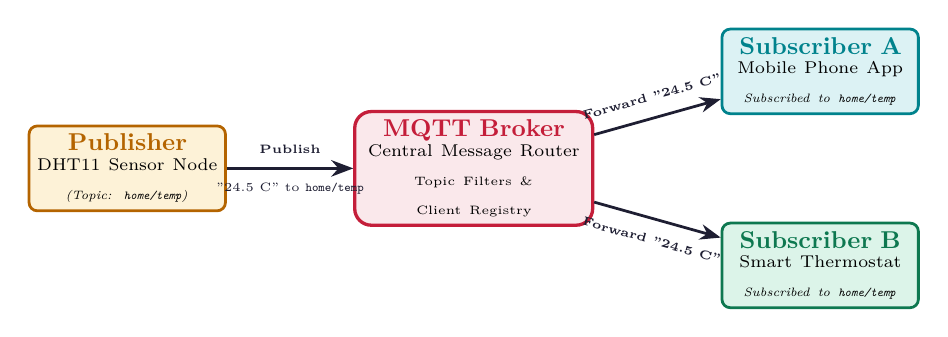
\begin{tikzpicture}[scale=0.88, transform shape]
  % Publisher (Left)
  \node[draw=myamber, fill=hdramber, rounded corners=3pt, line width=1pt, text width=2.6cm, align=center, minimum height=1.1cm] (pub) at (-5.0, 0) {
    \textbf{\color{myamber}Publisher}\\
    \scriptsize DHT11 Sensor Node\\
    \itshape\tiny (Topic: \texttt{home/temp})
  };

  % Broker (Center)
  \node[draw=myred, fill=hdrred, rounded corners=6pt, line width=1.2pt, text width=3.2cm, align=center, minimum height=1.3cm] (broker) at (0, 0) {
    \textbf{\color{myred}MQTT Broker}\\
    \scriptsize Central Message Router\\
    \tiny Topic Filters \& Client Registry
  };

  % Subscriber 1 (Top Right)
  \node[draw=myteal, fill=hdrteal, rounded corners=3pt, line width=1pt, text width=2.6cm, align=center, minimum height=1.1cm] (sub1) at (5.0, 1.4) {
    \textbf{\color{myteal}Subscriber A}\\
    \scriptsize Mobile Phone App\\
    \itshape\tiny Subscribed to \texttt{home/temp}
  };

  % Subscriber 2 (Bottom Right)
  \node[draw=mygreen, fill=hdrgreen, rounded corners=3pt, line width=1pt, text width=2.6cm, align=center, minimum height=1.1cm] (sub2) at (5.0, -1.4) {
    \textbf{\color{mygreen}Subscriber B}\\
    \scriptsize Smart Thermostat\\
    \itshape\tiny Subscribed to \texttt{home/temp}
  };

  % Connections - Straight and Sloped to avoid overlap
  \draw[arrow, line width=1.1pt] (pub) -- node[above=2pt, font=\tiny\bfseries] {Publish} node[below=2pt, font=\tiny] {"24.5 C" to \texttt{home/temp}} (broker);
  
  \draw[arrow, line width=1.0pt] (broker) -- node[midway, above=3pt, font=\tiny\bfseries, sloped] {Forward "24.5 C"} (sub1);
  \draw[arrow, line width=1.0pt] (broker) -- node[midway, below=3pt, font=\tiny\bfseries, sloped] {Forward "24.5 C"} (sub2);
\end{tikzpicture}
\end{tcolorbox}

\subsection{CoAP (Constrained Application Protocol)}
CoAP is a web transfer protocol designed for constrained nodes and networks:
\begin{itemize}[leftmargin=*, itemsep=2pt]
  \item It uses a RESTful request-response model mapping to standard HTTP methods (GET, POST, PUT, DELETE).
  \item Unlike HTTP, CoAP runs over \textbf{UDP} instead of TCP, dramatically reducing connection handshakes and packet overhead.
\end{itemize}

\begin{tcolorbox}[tikzbox, title={CoAP Request-Response over UDP}]
\centering
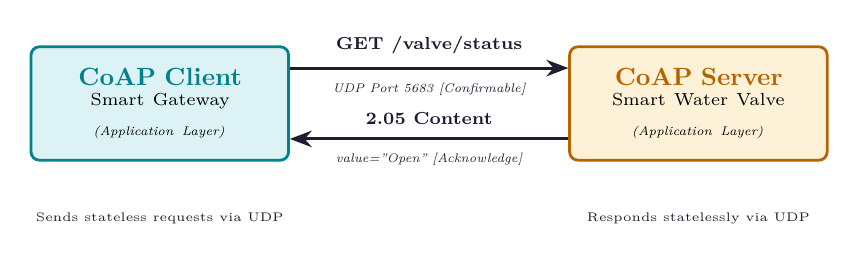
\begin{tikzpicture}[scale=0.9, transform shape]
  % Client Box
  \node[draw=myteal, fill=hdrteal, rounded corners=3pt, line width=1pt, text width=3.4cm, align=center, minimum height=1.6cm] (client) at (-3.8, 0) {
    \textbf{\color{myteal}CoAP Client}\\
    \scriptsize Smart Gateway\\
    \itshape\tiny (Application Layer)
  };

  % Server Box
  \node[draw=myamber, fill=hdramber, rounded corners=3pt, line width=1pt, text width=3.4cm, align=center, minimum height=1.6cm] (server) at (3.8, 0) {
    \textbf{\color{myamber}CoAP Server}\\
    \scriptsize Smart Water Valve\\
    \itshape\tiny (Application Layer)
  };

  % Communication flow lines - Increased gap to Y=+0.5 and Y=-0.5
  \draw[arrow, line width=1.1pt, color=mydark] ($(client.east)+(0,0.5)$) -- node[midway, above=2pt, font=\scriptsize\bfseries] {GET /valve/status} node[midway, below=2pt, font=\tiny\itshape, color=mydark] {UDP Port 5683 [Confirmable]} ($(server.west)+(0,0.5)$);
  
  \draw[arrow, line width=1.1pt, color=mydark] ($(server.west)+(0,-0.5)$) -- node[midway, above=2pt, font=\scriptsize\bfseries] {2.05 Content} node[midway, below=2pt, font=\tiny\itshape, color=mydark] {value="Open" [Acknowledge]} ($(client.east)+(0,-0.5)$);

  % Transport Layer Labels (Bottom)
  \node[below=0.6cm of client, font=\tiny, color=mydark] {Sends stateless requests via UDP};
  \node[below=0.6cm of server, font=\tiny, color=mydark] {Responds statelessly via UDP};
\end{tikzpicture}
\end{tcolorbox}

\newpage

% ═══════════════════════════════════════════════════════════════════════════════
% QUICK REVISION PAGE
% ═══════════════════════════════════════════════════════════════════════════════
\begin{center}
  {\large\bfseries\color{myred} Quick Revision — Module 2}\\[3pt]
  {\small\color{mydark} Networking \& Protocols $|$ OE-EC803A}
\end{center}
\noindent{\color{myred}\rule{\linewidth}{1.2pt}}
\vspace{8pt}

\begin{tcolorbox}[formulabox, title={\textbf{Key Protocols and Specs at a Glance}}]
\renewcommand{\arraystretch}{1.35}
\begin{tabularx}{\linewidth}{B{5.0cm} X}
  IPv4 Address Length & $32$ bits ($4$ bytes) $\rightarrow$ e.g., $192.168.1.10$ \\[4pt]
  IPv6 Address Length & $128$ bits ($16$ bytes) $\rightarrow$ e.g., $2001:0db8:85a3::8a2e:0370:7334$ \\[4pt]
  MQTT Ports & Port $1883$ (TCP, unencrypted) and Port $8883$ (Encrypted SSL/TLS) \\[4pt]
  CoAP Port & Port $5683$ (UDP, unencrypted) and Port $5684$ (DTLS security)
\end{tabularx}
\end{tcolorbox}

\vspace{6pt}

\begin{tcolorbox}[defbox, title={\textbf{One-Line Definitions}}]
\begin{itemize}[leftmargin=*, itemsep=3pt, topsep=0pt]
  \item \textbf{TCP/IP Model:} A standardized suite of communication protocols used to connect devices on the internet.
  \item \textbf{QoS (MQTT):} Quality of Service agreement determining the reliability and handshake level of message delivery.
  \item \textbf{MAC Address:} A permanent, unique physical address burned into the hardware interface card.
  \item \textbf{CoAP:} A lightweight RESTful transfer protocol running over UDP for constrained networks.
  \item \textbf{DHCP:} An automated protocol that dynamically assigns IP configurations to joining devices.
\end{itemize}
\end{tcolorbox}

\vspace{6pt}

\begin{tcolorbox}[exambox, title={\textbf{Frequently Asked / Viva Questions}}]
\begin{enumerate}[leftmargin=*, topsep=0pt, label=\textbf{Q\arabic*.}, itemsep=6pt]
  \item \Q{Why is TCP preferred for applications like web browsing, but UDP is preferred for real-time sensor streams?}
        TCP is connection-oriented and guarantees that every packet is received in order through acknowledgments. This prevents page layout distortion but adds latency. UDP sends packets without handshakes. It is faster, has less overhead, and is ideal for sensor streams where losing an occasional packet is acceptable but latency must be low.
        
  \item \Q{Why is IPv6 essential for the growth of IoT?}
        IPv4 only supports $4.3$ billion addresses, which have already been exhausted. IoT connects tens of billions of smart objects. IPv6 provides $128$-bit addresses ($3.4 \times 10^{38}$), allowing every individual device to have a globally unique IP address without routing behind NAT gateways.
        
  \item \Q{How does the publish-subscribe model in MQTT differ from the client-server model in HTTP?}
        In HTTP (client-server), clients pull data by initiating requests, requiring both devices to be online and active at the same time (tight temporal coupling). In MQTT (publish-subscribe), clients publish data to a broker, which pushes it to subscribers. The publisher and subscriber do not know each other and are decoupled.
        
  \item \Q{Explain the three QoS levels in MQTT.}
        (1) QoS 0 (At most once): Sends the message once with zero handshakes. Best for high-frequency, non-critical data. (2) QoS 1 (At least once): Delivers the message but might send duplicates. Requires a puback packet. (3) QoS 2 (Exactly once): Guarantees the message is received exactly once using a 4-packet exchange.
        
  \item \Q{What is CoAP, and what transport layer protocol does it use?}
        CoAP (Constrained Application Protocol) is a lightweight web transfer protocol designed for resource-constrained IoT nodes. It mirrors the RESTful model of HTTP (GET/POST) but runs over UDP, reducing header overhead and handshake latency.
        
  \item \Q{Why do we need a DNS server?}
        Humans read names (like `io.adafruit.com`), but routing hardware only reads binary IP addresses. The DNS server acts as a directory that looks up the domain name and returns the active IP address.
        
  \item \Q{Explain the difference between static and dynamic IP assignment.}
        Static IP addresses are configured manually and remain fixed, which is useful for local gateways. Dynamic IP addresses are leased temporarily from a pool by a DHCP server, which simplifies administration for large scale deployments.
        
  \item \Q{What is the difference between a MAC address and an IP address?}
        A MAC address is a physical, 48-bit identifier assigned permanently to the device hardware by the manufacturer. An IP address is a logical address assigned dynamically by the network to route packets across subnets.
\end{enumerate}
\end{tcolorbox}

\vspace{6pt}

\begin{tcolorbox}[tikzbox, title={\textbf{Comparison Snapshot}}]
\textbf{MQTT vs. CoAP vs. HTTP:}\par\vspace{6pt}\noindent
{\renewcommand{\arraystretch}{1.35}%
\begin{tabularx}{\linewidth}{|B{3.2cm}|Y|Y|Y|}
\hline
\textbf{Feature} & \textbf{MQTT} & \textbf{CoAP} & \textbf{HTTP} \\
\hline
Architecture & Publish / Subscribe & Request / Response (REST) & Request / Response (REST) \\
\hline
Transport Layer & TCP & UDP & TCP \\
\hline
Header Size & Minimal (2 bytes) & Small (4 bytes) & Large (Hundreds of bytes) \\
\hline
Security & SSL / TLS & DTLS & SSL / TLS (HTTPS) \\
\hline
Use Case & Continuous telemetry streams. & Low-power, event-driven queries. & Heavy dashboard interfaces. \\
\hline
\end{tabularx}}
\end{tcolorbox}

\end{document}
